\chapter{Protein Folding}

\say{\textit{la forma è l'immagine plastica	della funzione}}\footnote{\fullcite{ruffini1925fisiogenia}}\\

La correlazione tra forma e funzione si rivela fondamentale nel caso delle proteine. Un canale ionico neuronale permette il passaggio di ioni grazie alla sua forma a canale; una ferritina cattura e immagazzina gli ioni ferro grazie alla sua forma a sfera cava. 

\par Il ripiegamento delle proteine (\textit{protein folding}) è il processo di ripiegamento molecolare attraverso il quale a partire dalla sequenza lineare amminoacidica le proteine ottengono la loro struttura tridimensionale, chiamata forma \textit{nativa}, che permette loro di svolgere la relativa funzione biologica. Il ripiegamento nella forma tridimensionale avviene spontaneamente sia durante la sintesi proteica nei ribosomi sia al termine di questa. Una specifica proteina si ripiegherà nello stesso modo e avrà la stessa struttura finale\footnote{ciò non è vero nel 100\% dei casi, alcune proteine possono avere più di una conformazione stabile per adempiere funzioni diverse, vedi la sezione \ref{sec:fold-switching-proteins}}.

\par La prima teoria del ripiegamento proteico è stata proposta negli anni venti del 20° secolo da Hsien Wu\supercite{wu1931studies}, in relazione al processo di denaturazione (vedi sezione \ref{sec:denaturazione}). È però Anfinsen, premio Nobel per la chimica, negli anni '60 a compiere un fondamentale passo nella comprensione del processo del ripiegamento proteico\supercite{anfinsen1972formation}. 


\section{Postulato di Anfinsen}
Il postulato di Anfinsen (conosciuto anche come \textit{dogma} o \textit{ipotesi termodinamica} di Anfinsen) afferma che la struttura nativa delle proteine (almeno quelle globulari) è determinata solamente dalla sequenza di amminoacidi di cui sono costituite. In altri termini: la struttura nativa, in ambiente fisiologico standard, corrisponde a quella struttura unica, stabile e cineticamente accessibile avente \textit{minima energia libera}. 

\begin{figure}[h]
	\centering
	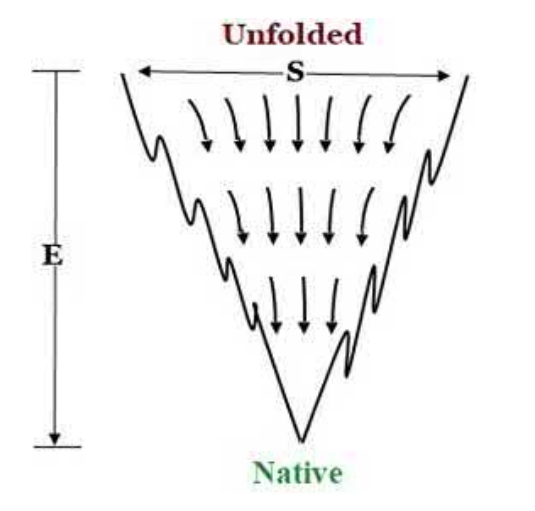
\includegraphics[scale=0.3]{images/funnel-folding.png}
	\caption{Un "panorama" idealizzato dell'energia libera a forma di imbuto. E=energia, S=entropia. Fonte: \cite{pal2019fundamentals}}
	\label{fig:funnel}
\end{figure}

Vi sono quindi 3 condizioni:

\begin{enumerate}
	\item \textit{unicità}, la sequenza non deve possedere altre configurazioni dotate di energia libera comparabile
	\item \textit{stabilità}, piccoli cambiamenti nell'ambiente circostante non possono produrre cambiamenti nella configurazione a energia minima. Ciò può essere descritto come una superficie parabolica di energia libera con lo stato nativo corrispondente al punto di minimo (visivamente simile ad un imbuto, vedi fig.\ref{fig:funnel}); la superficie di energia libera nelle vicinanze dello stato nativo deve essere abbastanza ripida ed elevata
	\item \textit{accessibilità cinetica}, il percorso nella superficie di energia libera dallo stato \textit{unfolded} a \textit{folded} deve essere ragionevolemente piano
\end{enumerate}


\subsection{Esperimento di Anfinsen}
L'esperimento, compiuto nel 1957\supercite{anfinsen1961kinetics}, consisteva nella denaturazione e rinaturazione della ribonucleasi A, dimostrando che il secondo processo era possibile senza agenti ausiliari. L'enzima in questione è formato da 124 amminoacidi, tra cui 8 cisteine che formano 4 ponti disolfuro ($-CH_{2}-\textbf{S-S}-CH_{2}-$). È stato usato un agente riducente per scindere questi ponti e l'urea per denaturare la proteina: questa non mostrava più alcuna attività enzimatica. A questo punto se l'urea era rimossa prima, seguita dall'aggiunta di un agente ossidante per consentire ai ponti disolfuro di riformarsi, la ribonucleasi A riacquistava spontaneamente la sua struttura terziaria e il prodotto ottenuto risultava praticamente indistinguibile dalla proteina nativa di partenza, riottenendo piena attività biologica. 

\begin{figure}[h]
	\centering
	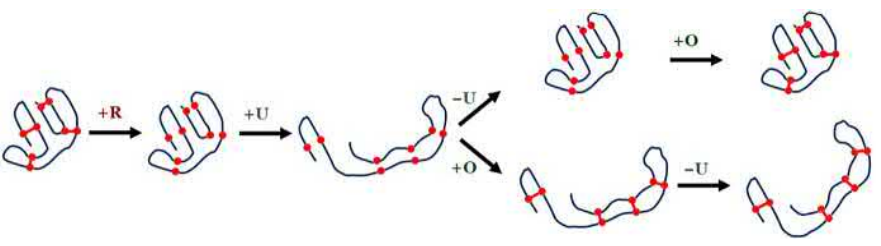
\includegraphics[scale=0.6]{images/anfinsen-experiment.png}
	\caption{Rappresentazione schematica dell'esperimento di Anfinsen. R=reducing agent, U=Urea, O=oxidizing agent, punti rossi=cisteina, linee rosse=ponti disolfuro. Fonte: \cite{pal2019fundamentals}}
	\label{fig:anfinsen-exp}
\end{figure}

I ponti disolfuro si riformano nella stessa posizione della proteina nativa nonostante ci siano 105 modi possibili per ricombinarli. Se invece veniva prima aggiunto l'agente ossidante e poi tolta l'urea il prodotto ottenuto era un miscuglio di molte delle possibili 105 configurazioni, raggiungendo solamente l'1\% dell'attività enzimatica.

\begin{figure}[!htb]
	\minipage{0.45\textwidth}
	\centering
	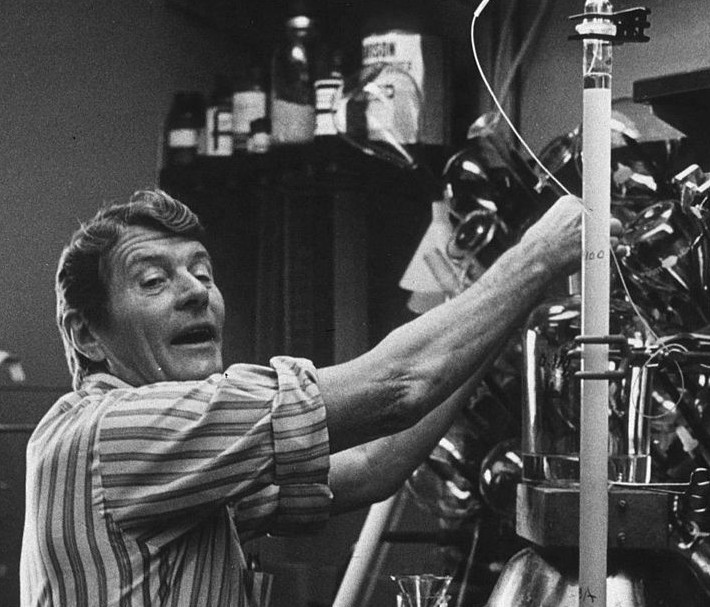
\includegraphics[scale=0.25]{images/anfinsen.jpg}
	\caption{C.B. Anfinsen nel suo laboratorio. Fonte: \cite{anfinsenNIH}}
	\label{fig:anfinsen}
	\endminipage\hfill
	\minipage{0.5\textwidth}
	\centering
	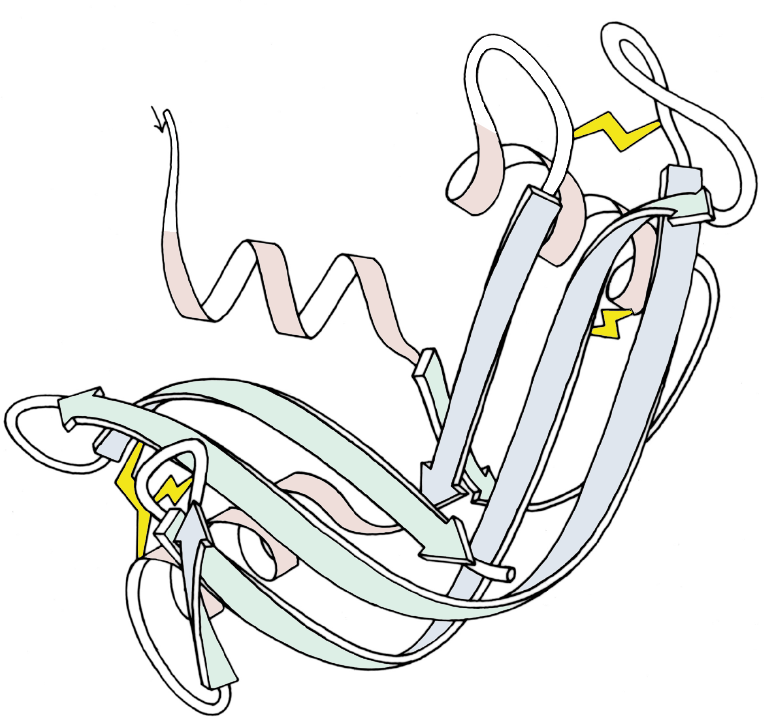
\includegraphics[scale=0.2]{images/RibonucleaseA_SS_paleRib.png}
	\caption{Ribonucleasi A, rappresentazione a nastro. In giallo i ponti disolfuro, rosa le $\alpha$-eliche, verde e azzurro i fogli-$\beta$. Fonte \cite{ribonucleasi-file}}
	\label{fig:ribonucleasi}
	\endminipage\hfill
\end{figure}

\subsection{Denaturazione} \label{sec:denaturazione}
La denaturazione delle proteine è il fenomeno relativo all'alterazione della struttura nativa dovuto a variazioni di temperatura, pH o contatto con determinate sostanze chimiche. La denaturazione è un processo che porta alla perdita di ordine e quindi ad un aumento di entropia. La struttura primaria rimane invariata, data la stabilità dei legami peptidici. A causa della denaturazione le proteine perdono la loro funzione biologica e possono esporre e rendere reattivi alcuni gruppi funzionali che possono causare l'aggregazione di più proteine. Può avvenire che una volta rimosso l’agente denaturante la proteina ritorni allo stato di partenza (\textit{rinaturazione}) ma spesso il processo è irreversibile.

\begin{figure}[h]
	\centering
	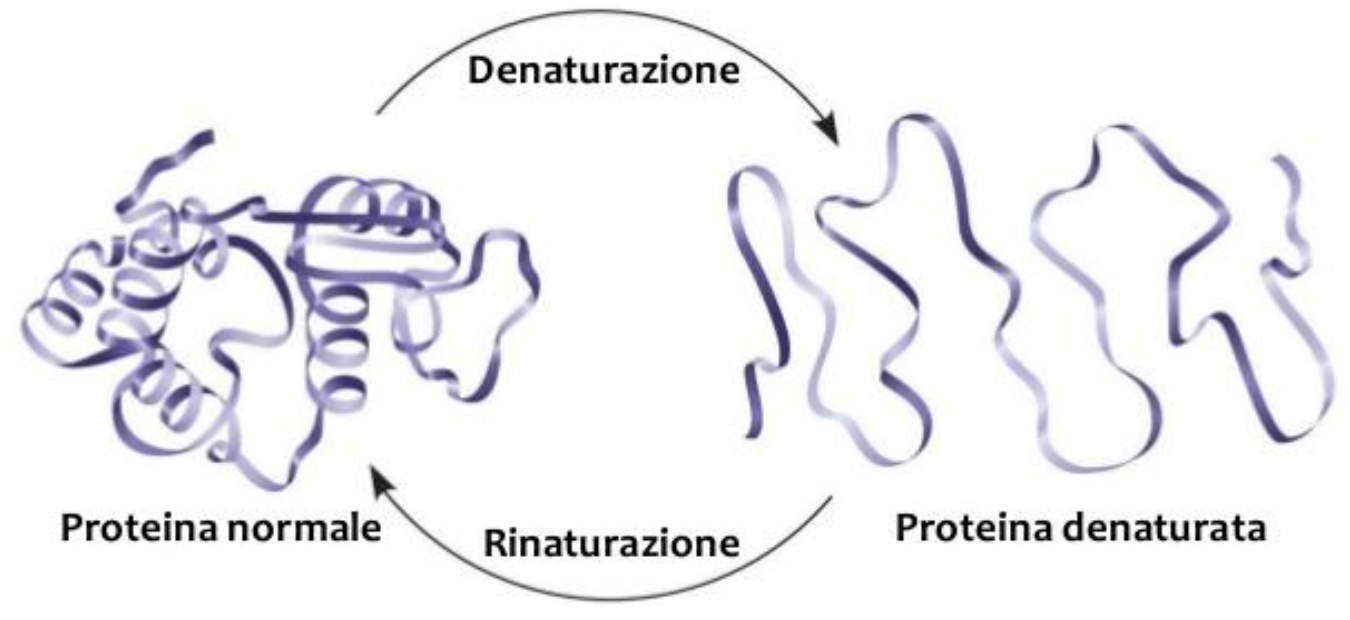
\includegraphics[scale=0.3]{images/denaturazione-rina.png}
	\caption{Denaturazione e rinaturazione. Fonte: \cite{campbell}}
	\label{fig:denaturazione}
\end{figure}

\par La proprietà di certe sostanze chimiche (es. urea) di denaturare una molecola proteica si deve alla loro capacità di legare transientemente, attraverso legami deboli, come ad esempio legami idrogeno, i residui amminoacidici costituenti la proteina. Questi legami vengono termodinamicamente preferiti a quelli intramolecolari o intermolecolari con l'acqua. Ciò comporta l'impossibilità per la proteina di mantenere la propria struttura tridimensionale e quindi questa si denatura. 

\par Applicazioni nella vita quotidiana di questo fenomeno sono la cottura dei cibi (basti pensare all'albumina nell'uovo) e la permanente ai capelli (denaturazione della cheratina, rompendo e riformando ponti disolfuro). 


\section{Struttura delle proteine}
\subsection{Interazioni molecolari}
\subsection{Struttura primaria}
\subsection{Struttura secondaria}
\subsection{Struttura terziaria}
\subsection{Struttura quaternaria}

• Domini, Residui, Motivi, Giri\\
• interazioni (covalenti, polari, van der Waals, ponti disolfuro, ..)\\
• una forza dominante o tante piccole forze?\\
• Cambio di paradigma da metà anni ‘80\\



-- strutture [ soft computing articolo]--
pri-
mary structure of proteins consist of linear sequences of twenty
natural amino acids joined together by peptide bonds. The sec-
ondary structure of a protein refers to the interactions due to
a regular arrangement of hydrogen bonds between CO and NH
groups (carboxyl and amino) of its amino acids, forming different
motifs ( ̨-helix, ˇ-sheet, loops and turns). The tertiary structure is
a description of the complex and irregular folding of the polypep-
tide chain in three dimensions. These complex structures are held
together by a combination of several molecular interactions (e.g.
ionic, hydrophobic or hydrogen bonds) that involve the amino acids
of the chain. The quaternary structure is the final dimensional struc-
ture formed by all the polypeptide chains making up a protein [13].

\section{Ripiegamento assistito}
All'interno delle cellule le proteine più piccole si ripiegano indipendentemente, mentre proteine più grandi sono assistite principalmente da complessi chiamati \textit{chaperoni molecolari}. È  importante notare che l'assistenza è cinetica in natura: non aggiunge nuove informazioni necessarie alla proteina per ripiegarsi, pertanto il dogma di Anfinsen non viene contraddetto. Ciò che fanno questi complessi è creare un ambiente nel quale le proteine possano ripiegarsi senza "distrazioni" dovute a interazioni con altre entità (ad esempio evitando l'aggregazione con altre proteine) e senza rimanere bloccate in conformazioni intermedie durante il loro percorso di ripiegamento. In poche parole sono misure di protezione della cellula. 

\begin{figure}[h]
	\centering
	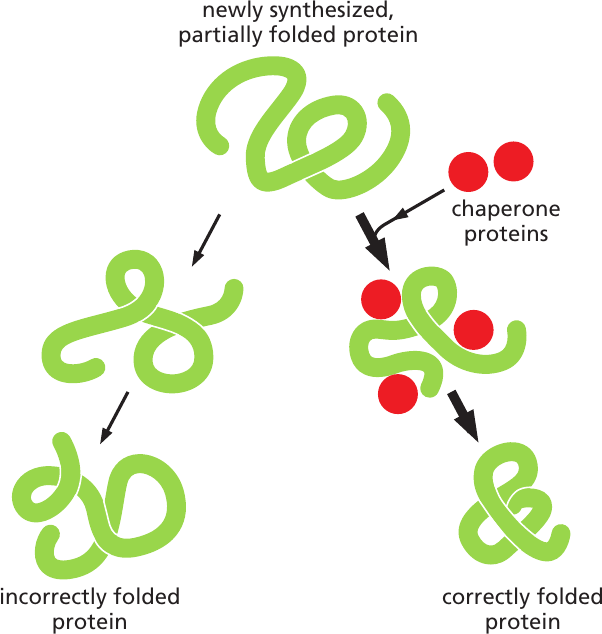
\includegraphics[scale=0.4]{images/chaperone-alberts.png}
	\caption{Schema della funzione dei chaperoni molecolari. Fonte: \cite{alberts2018essential}}
	\label{fig:chaperoni}
\end{figure}

Più in dettaglio i chaperoni molecolari svolgono le seguenti funzioni:
\begin{enumerate}
	\item assistono il corretto ripiegamento delle catene polipeptidiche (lunghe) appena sintetizzate
	\item dirigono l'assemblaggio di complessi multienzimatici
	\item donano una "seconda chance" a proteine danneggiate favorendone la rinaturazione
	\item partecipano nella parziale denaturazione durante il trasporto di proteine attraverso membrane di mitocondri o cloroplasti
\end{enumerate}

Tutti i compartimenti cellulari delle cellule eucariotiche (nucleo, citosol, reticolo endoplasmatico, mitocondri e cloroplasti) hanno il proprio set di chaperoni che assicura un corretto ripiegamento delle proteine. I chaperoni molecolari comprendono diverse famiglie di proteine altamente conservate, tra cui le Hsp (Heat shock protein), proteine espresse in grande quantità sotto condizioni di alto stress, per contrastare l'effetto denaturante del calore. Queste ultime sono state classificate in base al loro peso molecolare, ad es. Hsp60 dove "60" indica 60kDa. Le Hsp60 vengono chiamate anche \textit{chaperonine} e sono una famiglia di chaperoni molecolari a doppio anello che agiscono da "camera di isolamento" per il ripiegamento di altre proteine\supercite{ranson1998chaperonins}, famosa è la chaperonina procariotica GroEL (vedi fig.\ref{fig:groel}), che può essere assunta come modello di riferimento delle chaperonine. 

\begin{figure}[h]
	
\end{figure}

\begin{figure}[!htb]
	\minipage{0.35\textwidth}
	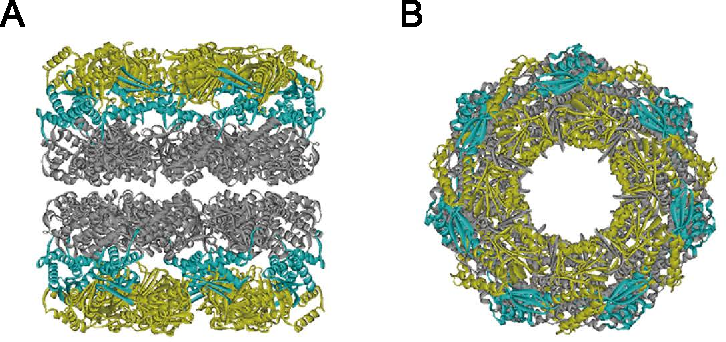
\includegraphics[scale=0.25]{images/groel.png}
	\caption{Strutture dei complessi GroEL e GroEL-GroES. (B) si può osservare la tipica forma ad anello. Fonte: \cite{Iizuka2016ChaperoninGU}}
	\label{fig:groel}
	\endminipage\hfill
	\minipage{0.6\textwidth}
	\centering
	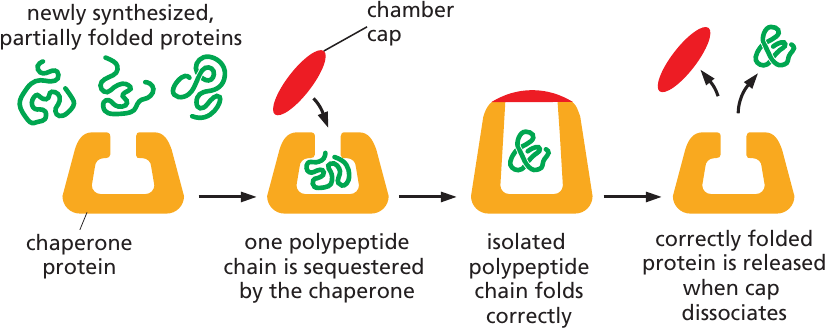
\includegraphics[scale=0.4]{images/chaperone-alberts-isolation.png}
	\caption{Rappresentazione schematica della funzione della camera di isolamento nelle chaperonine. Fonte \cite{alberts2018essential}}
	\label{fig:chaperone-camera}
	\endminipage\hfill
\end{figure}

Sebbene i mitocondri (e i clorplasti) abbiano il loro genoma e creino le loro proteine la maggior parte delle proteine usate in questi organelli sono codificate dai geni nel nucleo e importati dal citosol. Ogni proteina viene dispiegata per il trasporto. I chaperoni molecolari all'interno di questi organelli aiutano a tirare le proteine attraverso le due membrane e a ripiegarle una volta all'interno\supercite{alberts2018essential}.


\subsection{Misfolding e malattie}

Il \textit{misfolding} è il fenomeno dell'errato ripiegamento di una proteina, ovvero quando una proteina non può raggiungere il suo stato nativo. Ciò può accadere per mutazioni alla sua sequenza amminoacidica (come nel caso dell'anemia falciforme) o per fattori esterni.

L'errato ripiegamento delle proteine è alla base di molte patologie umane, definite malattie da misfolding, che possiamo dividere in due gruppi:

\begin{itemize}
	\item malattia causata dalla perdita o degradazione della proteina o dall'errato trasporto intracellulare
	\item malattie causate dall'accumulo, intra od extra-cellulare, di proteine aggregate (ad esempio le malattie da prione)
\end{itemize}

Molti tipi di tumore diventano chemio-resistenti perché iper-esprimono alcune Hsp, come la Hsp70 e la Hsp90. Le Hsp sono presenti anche in quantità elevatissime nel cervello dei pazienti con malattia di Alzheimer e morbo di Parkinson. Tuttavia si crede che la loro aumentata espressione non sia lesiva di per sé, ma rappresenti piuttosto una risposta difensiva agli elevati livelli di stress che caratterizzano queste patologie. Ci sono molti morbi associati a mutazioni nei geni codificanti i chaperoni. Alterazioni genetiche delle chaperonine possono portare a patologie umane che in genere colpiscono molti organi ed apparati contemporaneamente \supercite{chaperoninaWiki}. \\


neurodegenrative diseases
For example, prions are stable conformations of proteins which differ from the native folding state. In bovine spongiform encephalopathy, native proteins re-fold into a different stable conformation, which causes fatal amyloid buildup. Other amyloid diseases, including Alzheimer's disease and Parkinson's disease, are also exceptions to Anfinsen's dogma

-- misfolding [ soft computing articolo]--
Sometimes, a protein can fold into a wrong shape. A single miss-
ing or incorrect amino acid could cause such a misfold. As already
stated, protein function is determined by its structure, which can
be inferred from the sequence of amino acids, therefore a mis-
fold implies that a protein can not fulfill its function correctly.
Alzheimer’s disease, Cystic fibrosis and other neurodegenerative
diseases, mad cow disease are now attributed to protein misfolding (are associated with an accumulation
of misfolded proteins.). The knowledge
of the misfolding factors and understanding the protein folding
process, would help in developing cures for these diseases. There-
fore, the knowledge of the structure of the protein provides a great
advantage for the development of new drugs and the design of new
proteins.

- prioni

\subsection{Controllo qualità e proteasomi}
------
Exit from the ER Is Controlled to Ensure Protein Quality

 Some proteins made in the ER are destined to function there.
 Most proteins that enter the ER, however, are des-
tined for other locations; they are packaged into transport vesicles that
bud from the ER and fuse with the Golgi apparatus.
Exit from the ER is highly selective. 
Proteins that fail to fold correctly, and
dimeric or multimeric proteins that do not assemble properly, are actively
retained in the ER by binding to chaperone proteins that reside there. The
chaperones hold these proteins in the ER until proper folding or assembly
occurs. Chaperones prevent misfolded proteins from aggregating, which
helps steer proteins along a path toward proper folding (see Figures 4−8
and 4−9); if proper folding and assembly still fail, the proteins are exported
to the cytosol, where they are degraded by the proteasome, attraverso reazioni di proteolisi.

Le proteine da degradare sono contraddistinte dal loro legame con l'ubiquitina.

I proteasomi sono presenti nelle cellule di tutti gli eucarioti ed archea, nonché in alcuni batteri. La struttura e la funzione di questi complessi è altamente conservata, soprattutto tra le specie eucariotiche.

Per "la scoperta della degradazione delle proteine mediata da ubiquitina" è stato assegnato il Premio Nobel per la chimica del 2004 ad Aaron Ciechanover, Avram Hershko ed Irwin Rose.

A causa del ruolo dei proteasomi nella regolazione del ciclo cellulare e dell'apoptosi, sono oggi un bersaglio rilevante nelle terapie antitumorali. 

Antibody molecules, for example, are composed of four polypep-
tide chains (see Figure 4−33) that assemble into the complete antibody
molecule in the ER. Partially assembled antibodies are retained in the ER
until all four polypeptide chains have assembled; any antibody molecule
that fails to assemble properly is degraded. In this way, the ER controls
the quality of the proteins that it exports to the Golgi apparatus.

Sometimes, however, this quality control mechanism can be detrimen-
tal to the organism. For example, the predominant mutation that causes
the common genetic disease cystic fibrosis, which leads to severe lung
damage, produces a plasma membrane transport protein that is slightly
misfolded; even though the mutant protein could function normally as a
chloride channel if it reached the plasma membrane, it is retained in the
ER and then degraded, with dire consequences. This devastating disease
comes about not because the mutation inactivates an important protein
but because the active protein is discarded by the cells before it is given
an opportunity to function.


\subsection{Unfolded protein response}
The Size of the ER Is Controlled by the Demand for Protein Folding

Although chaperones help proteins in the ER fold properly and retain those
that do not, this quality control system can become overwhelmed. When
this happens, misfolded proteins accumulate in the ER. If the buildup is
large enough, it triggers a complex program called the unfolded pro-
tein response (UPR). This program prompts the cell to produce more ER,
including more chaperones and other proteins concerned with quality
control (Figure 15−25).
The UPR allows a cell to adjust the size of its ER to properly handle the
volume of proteins entering the secretory pathway. In some cases, how-
ever, even an expanded ER cannot keep up with the demand, and the
UPR directs the cell to self-destruct by undergoing apoptosis. Such a situ-
ation may occur in adult-onset diabetes, where tissues gradually become
resistant to the effects of insulin. To compensate for this resistance, the
insulin-secreting cells in the pancreas produce more and more insulin.
Eventually, their ER reaches a maximum capacity, at which point the UPR
can trigger cell death. As more insulin-secreting cells are eliminated, the
demand on the surviving cells increases, making it more likely that they
will die as well, further exacerbating the disease.

\section{Eccezioni al postulato di Anfinsen}

-- IDP [ soft computing articolo]---
The structure of some proteins is difficult to determine
for a simple reason: A growing body of biochemical research
has revealed that a significant number of proteins, or regions
of proteins, do not have a distinct 3-D structure until they
interact with a target protein or other molecule. Their flexibil-
ity and indefinite structure are important for their function,
which may require binding with different targets at different
times. These proteins, which may account for 20–30% of
mammalian proteins, are called intrinsically disordered proteins
and are the focus of current research.


\subsection{Intrinsically disordered proteins}

\subsection{Fold switching proteins} \label{sec:fold-switching-proteins}
Some proteins have multiple native structures, and change their fold based on some external factors. For example, the KaiB protein complex switches fold throughout the day, acting as a clock for cyanobacteria. It has been estimated that around 0.5–4\% of PDB proteins switch folds.[7] The switching between alternative structures is driven by interactions of the protein with small ligands or other proteins, by chemical modifications (such as phosphorylation) or by changed environmental conditions, such as temperature, pH or membrane potential. Each alternative structure may either correspond to the global minimum of free energy of the protein at the given conditions or be kinetically trapped in a higher local minimum of free energy.[8]


--- porter, youtube ---
“I study proteins and proteins have been thought to have one structure that has one function or fold. I'm studying this group of proteins called fold switching proteins. So, they can actually change their structures and their functions in response to changes in the cell. So, you can kind of imagine fold switching proteins are like a transformer where in one case the protein is like a robot that does one thing and then in another case, in response to changes in our bodies, it becomes a car and can do something else. And an advantage to this is it can respond really quickly to changes in our bodies

\subsection{box: Filosofia della scienza}


\section{Il problema del Protein Folding}
• cos’è il problema del protein folding: non solo la struttura finale\\
• 3 sottoproblemi: folding code, protein structure prediction e folding process\\
• le domande di principio del protein folding\\
- paradosso di Levinthal

\subsection{Limiti al ripiegamento}
• Limiti al ripiegamento: angoli di tersione e piano di Ramachandran\\

\subsection{Energetica del ripiegamento}
• processo spontaneo: energia di Gibbs, entalpia, entropia\\


--- Biochemists now know the amino acid sequence for about
160 million proteins, with about 4.5–5 million added each
month, and the three-dimensional shape for about 40,000.
Researchers have tried to correlate the primary structure of
many proteins with their three-dimensional structure to dis-
cover the rules of protein folding. Unfortunately, however,
the protein-folding process is not that simple. Most proteins
probably go through several intermediate structures on their
way to a stable shape, and looking at the mature structure
does not reveal the stages of folding required to achieve that
form

-- strumenti [ soft computing articolo]---
Even when scientists have a correctly folded protein in
hand, determining its exact three-dimensional structure is
not simple, for a single protein has thousands of atoms. The
method most commonly used to determine the 3-D structure
of a protein is X-ray crystallography

\begin{figure}[h]
	\centering
	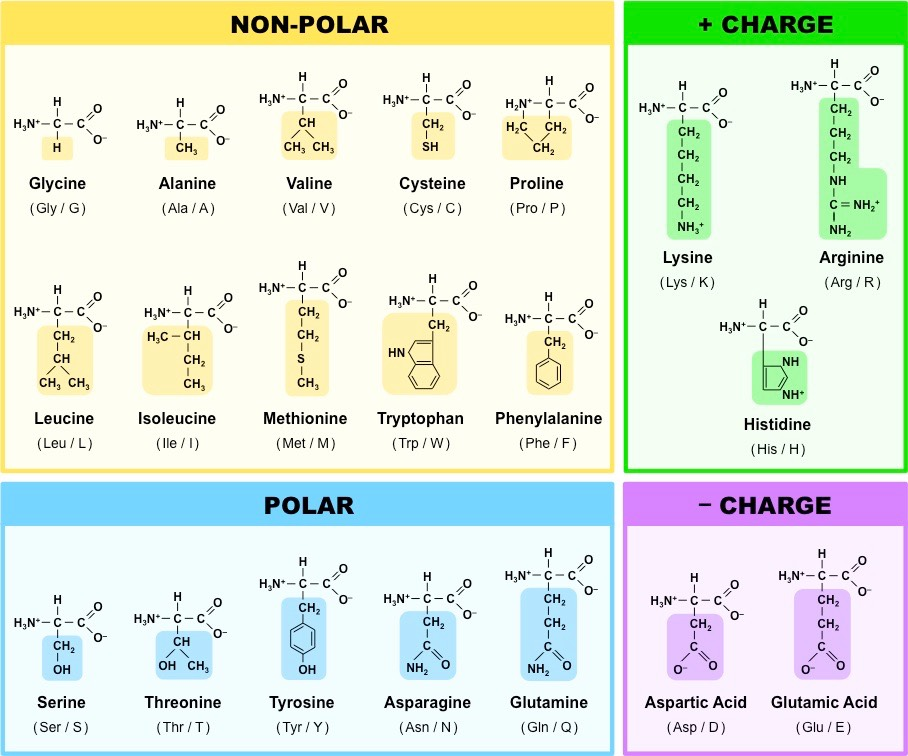
\includegraphics[scale=0.4]{images/aminoacid-tipi.jpeg}
	\caption{I 20 amminoacidi universali. Fonte: \cite{aminoacidTipi}}
	\label{fig:amminoacidi-tipi}
\end{figure}

\clearpage